% This is LLNCS.DEM the demonstration file of
% the LaTeX macro package from Springer-Verlag
% for Lecture Notes in Computer Science,
% version 2.4 for LaTeX2e as of 16. April 2010

%
\documentclass{llncs}
%

%TODO
%
% Conclusions
% Planning

\usepackage{makeidx}  % allows for indexgeneration

% Image Packages
\usepackage{graphicx}

\usepackage{caption}
\usepackage{subcaption}

\usepackage{float}
\captionsetup{compatibility=false}

\usepackage[space]{grffile}

% Llncs Packages
\usepackage{fixltx2e}

% UTF-8 Packages
\usepackage[utf8]{inputenc}

%
\begin{document}
%

%
\mainmatter              % start of the contributions
%

%
\title{Exploring Ray-Space Hierarchy on the GPU for Ray-Tracing of Dynamic Scenes}
%
\titlerunning{Exploring Ray-Space Hierarchy on the GPU for Ray-Tracing of Dynamic Scenes}  % abbreviated title (for running head)
%

%
\author{Nuno T. Reis}
%
\authorrunning{Nuno T. Reis} % abbreviated author list (for running head)
%
\tocauthor{Nuno T. Reis} % (use if author list has to be modified)
%

%
\institute{Instituto Superior Técnico, Portugal\\
\email{nunotiagoreis@tecnico.ulisboa.pt}\\}
%

\maketitle              % typeset the title of the contribution

\begin{abstract}

Over the last few years there have been great developments in the hardware for GPUs. GPGPU gained a lot of popularity as a consequence to these improvements
and many attempts are being made to adapt Ray-Tracing to the GPUs architecture. I am proposing an algorithm that runs fully on the GPU and that tries to maximize
its efficiency by taking advantage of the GPUs architecture. The algorithm consists of 5 main stages, rasterization, ray sorting, ray hierarchy creation, ray hierarchy
traversal and finally the local intersection tests. By combining ray sorting and a ray hierarchy my goal is to create a tight-fit structure that contains the scenes rays and
minimizes the number of local intersection tests, the main bottleneck in Ray-Tracing.

\keywords{Rasterization, Ray-Tracing, Ray-Sorting, Secondary Rays, Acceleration Structures, Object-Space, Bounding-Volume, Ray-Space, Ray-Bundling, Hierarchies, GPGPU}

\end{abstract}

%
\section{Introduction}
%

Ray-tracing is a global illumination technique used for the synthesis of photo-realistic images that involves ray-casting.
The first ray-casting algorithm was presented by Arthur Appel \cite{Appel68}, although it was only referred to as such until later on. 
This algorithm involved casting a set number of rays from the eye and intersecting those rays with the geometry composing the scene. 

\medskip

In 1979 Whitted \cite{Whitted80} presented a paper introducing a recursive ray-tracing algorithm, which is now known as Whitted Ray-Tracing. 
This algorithm, much like the original algorithm by Appel, casts rays from the eye but does not stop there. 
If the rays intersect geometry they can generate up to three different kinds of rays: shadow, reflection and refraction rays. These rays are also called secondary rays.

\medskip

Shadow rays are cast towards the light sources present in the scene. These rays are cast to check if the intersected object is being illuminated directly or if there are any other objects blocking the light source. 
Reflection rays are cast in a mirror-reflection direction. However, these rays are only cast if the intersected object has reflective properties. 
Refraction rays are cast through objects. This means that the intersected object must be translucent and that the refraction direction also depends on the material of both the rays current and next travel mediums refraction index.

\medskip

These rays differentiate ray-tracing from rasterization since they allow realistic and complex effects like reflections, refractions and shadows. This does not come without a price however. Ray-tracing is very inefficient and up to this day there has been extensive research to try and optimize it. Most of this research involves creating hierarchies in both Ray and Object space. 

\medskip

In Naive Ray-Tracing each ray is tested against each polygon in the scene, which leads to N x M intersection tests per frame, assuming that we have N rays and M polygons. This isn't feasible, especially with moderately complex scenes. To optimize this naive approach (and Ray-Tracing in general) there are two common approaches that try to reduce the number of intersection tests, the bottleneck of the algorithm. Whitted suggested the use of bounding volumes to achieve this goal.

\medskip

One of these two approaches involves using Object-Space Hierarchies, which help reduce the number of intersections by creating a structure encompassing the scenes geometry that allows the scenes to be tested for intersections without actually testing every single polygon. These techniques usually have problems handling dynamic scenes since this forces the hierarchies to be rebuilt each frame. In the past few years many developments have been made in this area with significant results.

\medskip

The other approach uses Ray-Space Hierarchies to achieve the same goal, to reduce the number of intersections. Instead of creating hierarchies based on the scenes geometry, they are based on the rays being cast in each frame. One of the solutions is ray-bundling, which consists in grouping several rays together and intersecting the bundle of rays with the geometry. This saves many intersection tests because if a bundle does not intersect any geometry then the rays in said bundle don't need to be tested any more in that particular frame. Another solution involve caching of rays, for example using 5D tuples to represent them. In these solutions the rays are represented as hypercubes in 5D space, which are then intersected with the scenes geometry. These intersection results are then cached and used to reduce future intersection tests for new rays.

\medskip

Over the last few years many improvements have been made in both Object-Space and Ray-Space approaches. The development of General-purpose computation on Graphic Processing Units (GPGPU) over the past years has led to many attempts to implement Ray-tracing on the GPU. This is no trivial task however. Modern GPUs are composed of Single instruction, Multiple data units (SIMD), which means that they are optimized to repeat the same operations over large sets of input. Ray-tracing by nature isn't easily mapped onto GPUs since each ray can generate secondary rays, but it also might not do so, which is a problem since each ray-cast (even for very similar rays, in both origin and direction) has the potential to have a different number of bounces and even hit different triangles.

\medskip

In this report I will analyze three different approaches based on ray-space hierarchies, one using caching mechanisms, one using ray bundles combined with a tree hierarchy and one using ray sorting combined with ray bundles. Finally I will propose an improvement to the ray-bundle approach by Roger et al. \cite{Roger07}, combining it with the ray-sorting approach by Garanzha and Loop \cite{GaranzhaLoop10} to achieve higher efficiency in the ray-object intersection tests. This ray-bundling approach will also be parallelized so that it is mapped more efficiently on the GPU, leading to better performance.

%
\section{Objectives}
%

This work aims to implement an algorithm for Interactive Whitted Ray-Tracing that is capable of rendering dynamic scenes in real-time on the GPU, while focusing on the secondary rays. This will be done by reducing the Ray-Triangle intersection tests, which is the bottleneck of Whitted Ray-Tracing and adapting Ray-Tracing to GPGPU, which is not a trivial task.

%
\subsection{Find the State of the Art}
%

In order to implement an algorithm capable of what was described in the paragraph above it is necessary to research what are the techniques being used today. This research should serve as a base for the development of the algorithm.

%
\subsection{Choosing and Improving the approach}
%

After researching the State of the Art an approach should be chosen keeping in mind that it should be flexible enough to allow for improvements. These improvements should focus on reducing the number of intersection tests, or in other words, focus on the efficiency of the Ray-Tracing algorithm.

%
\subsection{Preliminary Analysis}
%

Finally it is necessary to evaluate the proposed algorithm. A preliminary analysis should show if the algorithm is indeed completing the objective even if it is just an initial version.

%
\section{Previous Work}
%

In this section I will focus on previous research in Ray-Space Hierarchies.Not all of these papers are focused on interactive Ray-Tracing. However it is still helpful to find out which approaches were tried before and why they couldn't be used in the development of my algorithm. I will also go over a few parallel scan and sorting algorithms since these are necessary for the improvements that I plan to introduce.

%
\subsection{Fast Ray Tracing by Ray Classification}
%

Arvo and Kirk \cite{ArvoKirk87} introduced a 5-dimensional ray-space hierarchy. They subdivided the ray-space in such a way that all relevant rays are distributed among equivalence classes. These classes are associated with a candidate object set. For example, the candidate set C\textsubscript{i} contains the objects that the rays in the equivalence class E\textsubscript{i} can intersect. The focus of this algorithm is to decrease the number of intersection tests.

\medskip

Since this algorithm works in a 5-dimensional space, the first thing we need to know is which are the degrees of freedom that a ray actually has. Traditionally rays are represented by a point and a vector in a 3-dimensional space, representing its origin and its direction. However a ray only has 5 degrees of freedom. These 5 degrees are its origin, which accounts for 3 degrees, and its direction, which accounts for 2 degrees when using spherical coordinates. This allowed Arvo and Kirk to parametrize rays and thus create subsets of the rays 5-dimensional space in such a way that rays with similar origins and directions would be in the same subset. 

\medskip

The algorithm was broken into these 5 steps that I will now describe. It is also important to note that the first step is only carried out once while the second and third steps are consistently carried out in order to refine the hierarchy.

\subsubsection{Bounding Volume Creation}

The first step is to find the 5-dimensional bounding volume that contains the equivalent of each ray that can interact with the environment in said space. Since it's important to use volumes that don't take up too much space they chose to store 5 ordered pairs that represent intervals in the 5 orthogonal axes, which they labeled x,y,z,u and v. These 5 ordered pairs represent a bounding volume. Each of these bounding volumes, denominated hypercubes, have a representation in 3-dimensional space which they call a beam. This is vital to the algorithm because this beam comprises the points in 3-dimensional space that the set of rays contained in the hypercube can reach. One of the issues however is that the beams associated with the hypercubes are not generally polyhedra. To account for this fact, they used 6 different mappings that have the desired properties locally and together contain the whole ray-space. Each of the 6 mappings correspond to a dominant axis, x+,x-,y+,y-,z+ or z-, and one sixth of the direction space. The bounding volume is then created by creating six copies of the bounding volume created from the bounding box containing all the geometry. The rays are then mapped onto these bounding volumes.

\subsubsection{Space Subdivision}

The second step is to subdivide the 5-dimensional space into equivalence classes. The smaller each hypercube is, the more likely rays are to behave coherently. However, the smaller each hypercube is, the more classes we will have. The goal is to have hypercubes sufficiently small so that the rays of the corresponding beams intersect approximately the same objects, allowing the rays in that beam to share a set of candidate objects. Starting with the 6 bounding volumes created earlier, the hierarchy is created by subdividing each hypercube in half at each level, cycling each of the 5 axis. This continues until either the hypercubes size or the sets number of candidate objects fall below a fixed threshold. It is important to note that hypercubes are only subdivided if they contain rays generated during the ray-tracing process.

\subsubsection{Candidate set Creation}

For the third step each objects bounding box is intersected with the beam associated with the hypercube being tested. If there is an intersection then the object is added to that hypercubes candidate set. As the space is subdivided the candidate sets for the child hypercubes must be updated. Since there is an overlap between parent and child hypercubes they found that re-evaluating the candidate sets should only be done only after the hypercubes have been divided on all of the 5 axis, meaning a re-evaluation only after 5 subdivisions have occurred.

\subsubsection{Ray Classification}

The fourth step consists of finding the 5-dimensional hypercube that each ray corresponds to. This is done by mapping the ray to the 5-dimensional space and then traversing the ray-space hierarchy, beginning with the hypercube that is indexed by the rays dominant axis (this hypercube is one of the 6 copies created at the start of the algorithm) until the leaf containing the ray is reached. If the candidate set corresponding to this leaf is empty then the ray intersects nothing. Otherwise, we proceed to the next step.

\subsubsection{Intersection Tests}	

Finally the ray is tested with each object for intersections. Initially a coarse intersection test is carried out by using the objects bounding volume instead of the actual object, in order to reject rays that don't intersect the object.

\subsubsection{Considerations}

This algorithm works similarly to a Hash Tree, in the sense that each ray is converted to a key (in this case the corresponding 5-dimensional point) and after finding out which class it belong to (the classes can be associated with the equivalence classes) it is then mapped to a value (in this case the candidate object set). For dynamic scenes it would be necessary to recalculate the candidate sets each time the objects moved, which would be very costly. This means that the ray-space hierarchy is tightly connected to the objects and their positioning in the scene. This suggests that the algorithm is not a very good fit for ray-tracing of dynamic scenes, which is my goal.

%
\subsection{Five-dimensional Adaptive Subdivision for Ray Tracing}
%

Simiakakis and Day \cite{SimiakisDay94} introduced some improvements to Arvo and Kirks work \cite{ArvoKirk87}. These improvements consist of using a directional subdivision method, which adapts automatically according to the scene. They also introduced a memory saving scheme but the main issues with Arvo and Kirks paper with dynamic scenes still remain, which does not make this algorithm a good fit for dynamic scenes.

%
\subsection{Whitted Ray-Tracing for Dynamic Scenes using a Ray-Space Hierarchy on the GPU}
%

Roger et al. \cite{Roger07} presented an algorithm for interactive rendering of animated scenes with Whitted Ray-Tracing. This algorithm ran fully on the GPU and focuses on the secondary rays, using the GPU rasterizer to process the primary rays. They use a ray-space hierarchy that bundles rays together using cones and spheres. The algorithm is mapped on the GPU using textures to pass information between each of the algorithms phases.

\medskip

The algorithm consists of 5 steps that i will describe. It is important to keep in mind that the first step uses the GPU rasterizer since it has the same effect as tracing the primary rays but rasterizing them is faster.

\subsubsection{Render the Scene using the Rasterizer}

This step is done using the traditional rasterizer (for example using modern OpenGLs rasterization pipeline) that outputs the pixel color, without any kind of secondary ray effects like shadows,  reflections and refractions. Like it was stated  before, the primary rays give us the same pixel color as the standard rasterizer, so they took advantage of the performance of the rasterizer to speed-up the algorithm.

\subsubsection{Generate the first set of Secondary Rays}

Since fragment shaders can have multiple render targets, they take advantage of this fact to output the initial set of secondary rays as well. These rays can consist of the shadow rays, reflection rays and refraction rays.. Since the algorithm is generic enough, it does not matter which kind of secondary rays are used. It is also worth noting that the shadow rays are very coherent locally (if we're using soft shadows) so they fit cone hierarchy quite well.

\subsubsection{Build the Ray-Space Hierarchy}

The second step is taking the rays generated from the previous step and constructing the hierarchy. Each node consists of a structure composed by a sphere and a cone, which means that 8 floats are stored, 3 for spheres center and 1 for the spheres radius, 3 for the cones direction and 1 for the cones spread angle.i The hierarchy is constructed bottom-up, meaning that the leaves are constructed first. These leaves consist of spheres with radii 0 and cones with spread 0, representing the exact rays. The upper levels are then constructed by computing the union of the child nodes until we have a top node that encloses the whole ray-space.

\subsubsection{Intersect the Ray-Space Hierarchy with the Scene}

In this step the ray-space hierarchy is intersected with the scene. This is done in a top-down manner, testing each parent node before going down the hierarchy. Only triangles that intersect the parent node will be tested for intersections with the children nodes. This means that at each level of the hierarchy several triangles are removed from the intersection tests. It is also important to note that for this preliminary intersection phase the tests are carried out using the triangles bounding spheres since they are simply exclusion tests before the final local intersection tests. At each level of the hierarchy the intersection information is stored in textures, one for each of the 4 children nodes. If there is an intersection, the IDs for the triangle and the cone are stored in a texture, otherwise an empty element is stored. Since the texture will have blanks when there are failed intersection tests. These 4 textures also need pruned of empty elements  for the next pass.

\medskip

This has two purposes, one being memory management and the other being the mapping of the algorithm to the GPGPU. Since each pass stores its output in textures we can process each pass using the same operations meaning that there won't be threads having different execution paths which in turn is one of the features necessary to make an algorithm fit the GPU. These pruning methods are called stream-reduction passes and they presented two different methods, one involving an hierarchical version of Horns \cite{Horn05} and a slower one using geometry shaders. The hierarchical version works by breaking down the textures in components of fixed size and concatenating them at the end.

\subsubsection{Final Intersection Tests}	

Finally after traversing the hierarchy we have a texture with the triangle and  ray IDs (the last level of the hierarchy are individual rays), which means we need to calculate the traditional intersection tests, keeping the closest intersection.

\subsubsection{Considerations}

This algorithm works as a bounding volume hierarchy of sorts, adapted to the rays, using cones and spheres to enclose the ray bundles. It is also very well adapted to GPGPU since each pass has a fixed number of operations and has the same execution path. The stream-pass reduction method is vital since it helps prune the textures of empty elements, allowing the threads processing the textures to execute the same operations. Finally it leaves the possibility of combining the ray-space hierarchy with a object-space hierarchy, possibly reducing the number of intersections even more. It is also an example of hybrid rendering since it uses the GPUs rasterizer to compute the initial rays and the initial set of secondary rays.

%
\subsection{Fast Ray Sorting and Breadth-First Packet Traversal for GPU Ray Tracing}
%

Garanzha and Loop \cite{GaranzhaLoop10} introduced an algorithm using various parallel primitives to adapt the ray-tracing algorithm to the GPU. Their algorithm sorts the generated rays and creates tight-fit frustums on the GPU and then intersects them with a Bounding Volume Hierarchy for the scenes geometry that is built on the CPU. One of the most interesting parts of their work is the fast ray sorting since it is done using parallel primitives which mitigates the overall cost of the operation when its executed on the GPU. I will now go into more detail regarding the four stages of the algorithm that they outlined.

\medskip

\subsubsection{Ray Sorting}

The first step, Ray Sorting, is used to store coherent rays in coherent memory locations in order to have less divergence during the tracing routine. If any given set of rays are coherent, they are more likely to intersect the same geometry and thus access the same memory locations. The sorting also allows the frustums in the next step to be tighter fits and thus give us a smaller set of intersection candidates.

\medskip

To sort the rays, they created a key-index pair for each ray, with the key being the rays ID and the index being the rays Hash value. This hash value is computed by quantizing the rays origin in a virtual grid that is within the scenes bounding box and then by quantizing its direction using a similar process.
After creating this pair for every ray, a compression-sorting-decompression scheme is used. This compression step generates chunks out of the initial set of rays. These chunks are represented by three arrays, the hash array (which indicates hash each chunk), the base array (which indicates the index of the first ray in each chunk) and a size array. This compression step takes advantage of the fact that it is likely that rays that are generated sequentially will have the same hash value. These chunks are then sorted using radix sort. The final step is the decompression, which applies an exclusive scan on the chunks size array to generate an array that indicates where each chunk will start in the re-ordered rays set.
After the exclusive scan two arrays are generated, the skeleton array that contains the base of the chunk in the positions from which the re-ordered rays set will be created from and the head flags array that indicates where new chunks start. An inclusive segment scan is then applied to these two arrays and the final re-ordered ray set is built. The final part of the decompression step is extracting the ranges of the packets of coherent rays. This is done by compressing the re-ordered ray set, using the same procedure that was used for the un-ordered ray set and then dividing those compressed chunks into packets, with a maximum size that is defined manually and then by decompressing using an inclusive segmented scan once more.

\subsubsection{Frustum Creation}

The frustum creation step picks up where the sorting left off. From the packet ranges calculated in the previous step a frustum is created for each one, using a dominant axis and two axis aligned rectangles to represent them, bounding each ray in the packet.

\subsubsection{Frustum Traversal}

The frustums are then intersected with the scenes Bounding Volume Hierarchy that was created on the CPU. This binary BVH has arity eight and 2/3rds of the tree levels are eliminated and an Octo-BVH is created. After traversing the BVH in a breadth-first order, each frustum will have a list of leaves assigned to it, which contain the primitives that will be used in the next step.

\subsubsection{Local Intersection Tests}

Finally the leaves are iterated on and for each of the primitives that they contain, localized intersection tests are calculated.

\subsubsection{Considerations}

This algorithm does not create a global Ray-Space hierarchy that contains every single ray. Instead, smaller local Frustums are created, taking advantage of the Ray-Sorting step to make them tight-fits. This reduces the number of leaves that each frustum will have assigned to it after traversing the Bounding Volume Hierarchy, which in turn reduces the number of localized intersection tests. The Ray-Sorting step is very interesting as it uses parallel primitives such as segmented scans to maximize its effectiveness on the GPU.

%
%\subsection{Efficient Parallel Scan Algorithms for GPUs}
%

%\subsubsection{Parallel Scan}

%\subsubsection{Segmented Scan}

%\subsubsection{Considerations}

%
%\subsection{Designing Efficient Sorting Algorithms for Manycore GPUs}
%

%\subsubsection{Parallel Scan}

%\subsubsection{Segmented Scan}

%\subsubsection{Considerations}

%
\section{Proposed Algorithm}
%

After analyzing several papers I've decided to combine two approaches. The Ray-Space Hierarchy by Roger et al. \cite{Roger07} is very interesting and easy to build. It takes advantage of the properties of the cone and sphere used to represent nodes to create a structure that fits very well with rays, making it easy to construct the hierarchy while also fitting very well with the architecture of modern GPUs. It is also worth remembering that they used rasterization to render the primary rays, since the visual benefits of Ray-Tracing are acquired only after we trace the secondary rays. However, since the secondary rays are also incoherent it also means that they hierarchy has the potential of becoming very loose when rays that aren't similar at all  in both origin and orientation. This is an issue because the early traversal of the hierarchy will wield larger local intersection candidate sets. This means more local intersection tests overall, which is in fact what are are trying to reduce, since the intersection tests are the bottleneck of Ray-Tracing. By combining the Ray-Sorting approach taken by Garanzha and Loop \cite{GaranzhaLoop10} we can create clusters of coherent rays. With these clusters of coherent rays the local intersection candidate sets will be smaller which means we will calculate less intersections and thus improve the algorithms efficiency. I will now describe the algorithms individual steps from the perspective of a OpenGL and CUDA implementation.

\begin{figure}
\centering
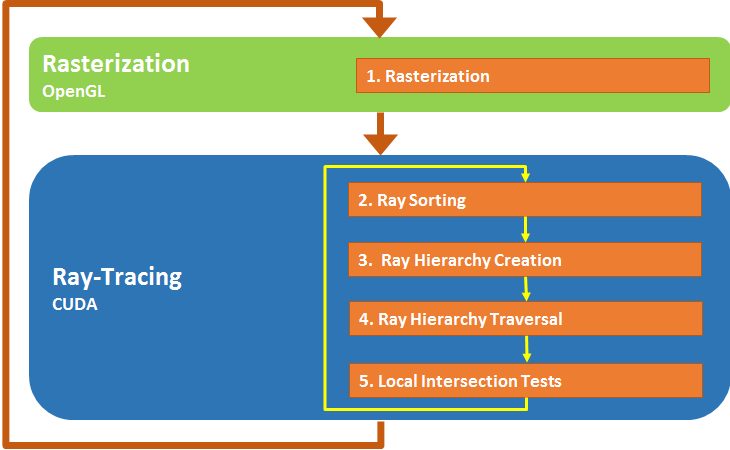
\includegraphics[scale=0.50]{images/figure 1.png}
\caption{Algorithm Overview.}
\end{figure}

%
\subsection{Rasterization}
%

The first step of the algorithm is the Rasterization. For the past years it was often generalized that Rasterization and Ray-Tracing were polar opposites and that a choice had to be 	made between the two despite this not being true at all. Although Rasterization is completely different from Ray-Tracing, one can complement the other. The first set of rays, the primary rays, does not convey any of the visual effects that Ray-Tracing is used for, such as Shadows, Reflections and Refractions. This means that Rasterization as we know it conveys the same effects as the tracing of the primary rays, while being extremely faster. If we complement the Rasterization of the primary rays with the Ray-Tracing the secondary rays we can get the benefits from both techniques, the efficiency of Rasterization and the visual effects from Ray-Tracing.

\medskip

This means however that the output from the fragment shaders used to rasterize the scene is more than just the traditional fragment colors. We need to create different render targets according to the information we want to store but in general we need to output the shadow, reflection and refraction rays. While being dependent on the implementation details it can be generalized that the fragment shader has to output 4 different textures, one consisting of the traditional 32 bit integer that will contain the pixel colors and three more consisting of two 32 bit floats that will contain the rays origin and direction for the shadow, reflection and refraction rays. These textures will then be accessed by the CUDA Kernel to read the information necessary to sort the secondary rays.

\begin{figure}
\centering
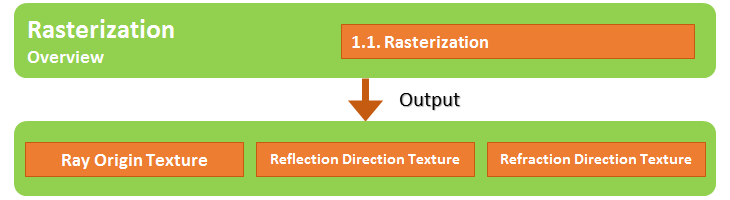
\includegraphics[scale=0.60]{images/figure 2.png}
\caption{Rasterization Overview.}
\end{figure}

\vspace*{-20pt}

\newpage

%
\subsection{Ray Sorting}
%

In this section I will describe in detail how each Ray-Sorting step works, based on the paper by Garanzha and Loop \cite{GaranzhaLoop10}.

\begin{figure}
\centering
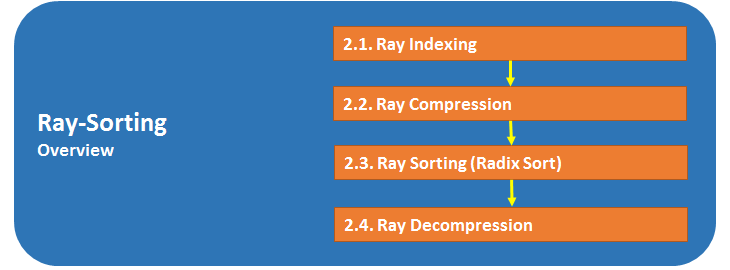
\includegraphics[scale=0.60]{images/figure 3.png}
\caption{Ray-Sorting Overview.}
\end{figure}

\vspace*{-20pt}

%
\subsubsection{Ray Indexing}
%

After rasterizing the scene and calculating the secondary rays we need to sort those secondary rays so that we can create clusters of coherent rays. To sort them first we need to assign a key-index pair to each ray. The index is quite simple since it only refers to the rays index in the corresponding ray texture. The key however is trickier since we need a way to compare rays using these keys. The solution from Garanzha and Loops work \cite{GaranzhaLoop10} is to quantize the rays origin and direction. The origin is quantized by partitioning the scene bounding box into a virtual grid with uniform cell size and then by calculating in which cell the rays origin is. The direction is quantized by creating an angular partition centered on the rays origin and then by calculating the section to which the rays direction is pointing to. Once we have these two values we merge them into a 32bit integer and we can use that integer as the key. With the keys and the indices we create an array containing a pair for each secondary ray. An example of this partitioning can be seen in figures~\ref{fig:directional-partitioning} and~\ref{fig:spatial-partitioning} below.

\begin{figure}
\centering
\begin{minipage}{.5\textwidth}
  \centering
  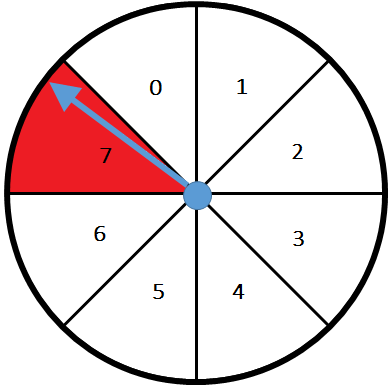
\includegraphics[width=.45\linewidth]{images/figure 7.png}
  \captionof{figure}{Directional Partitioning - 2D}
  \label{fig:directional-partitioning}
\end{minipage}%
\begin{minipage}{.5\textwidth}
  \centering
  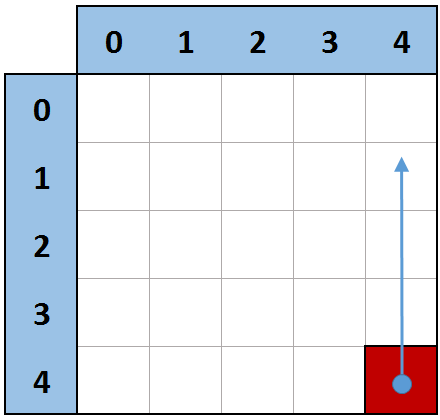
\includegraphics[width=.45\linewidth]{images/figure 8.png}
  \captionof{figure}{Spatial Partitioning - 2D}
  \label{fig:spatial-partitioning}
\end{minipage}
\end{figure}

%
\subsubsection{Ray Compression}
%

After creating the key-index pairs we need to sort them using a compression-sorting-decompression scheme. The compression step exploits the local coherency of rays. Even for secondary rays, the bounces generated by two adjacent rays have a good chance of being coherent which can result  in the same hash value for both bounces. With this information in mind, we compress the key-index pairs into chucks effectively minimizing the number of pairs that need to be sorted. To compress the pairs we create a head flags array with the same size as the key-index pair array, initializing it with 0s in every position. We then insert a 1 in the indices in which the hash value of the corresponding pair differs from the previous pairs. After creating the head flags we apply an exclusive scan operator on it. By combining the head flags array and the scan output array we can create the chunk hash, base and size arrays, which contain the hash, starting index and size of the corresponding chunks (see figure~\ref{fig:ray-compression} below).

\begin{figure}
\centering
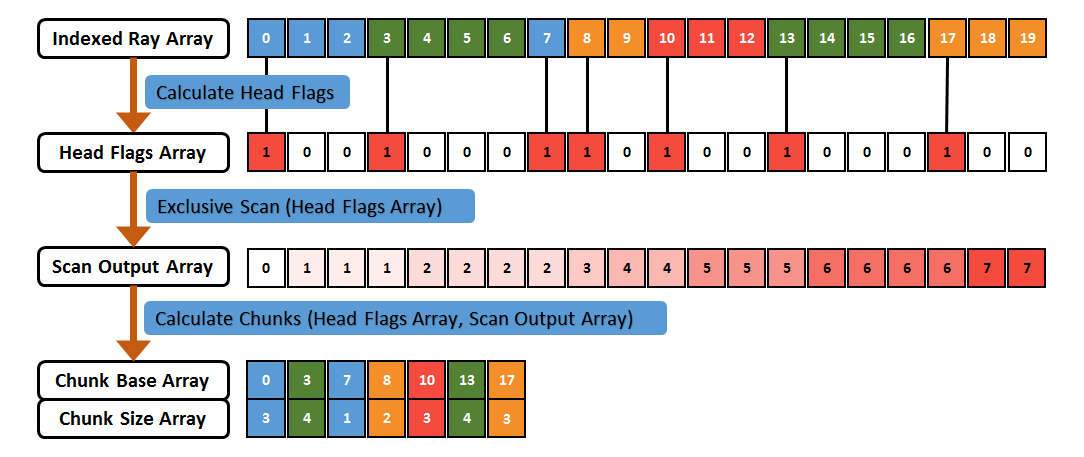
\includegraphics[scale=0.45]{images/figure 10.png}
\caption{Ray Compression into Chunks using parallel primitives.}
\label{fig:ray-compression}
\end{figure}

\vspace*{-30pt}

%
\subsubsection{Ray Sorting}
%

By this time we have an array of chunks with the information necessary to reconstruct the initial array of rays and we can begin the actual sorting. By using radix sort \cite{Satish09} on the array of chunks we will get a new array of chunks sorted according to the rays quantization.

\begin{figure}
\centering
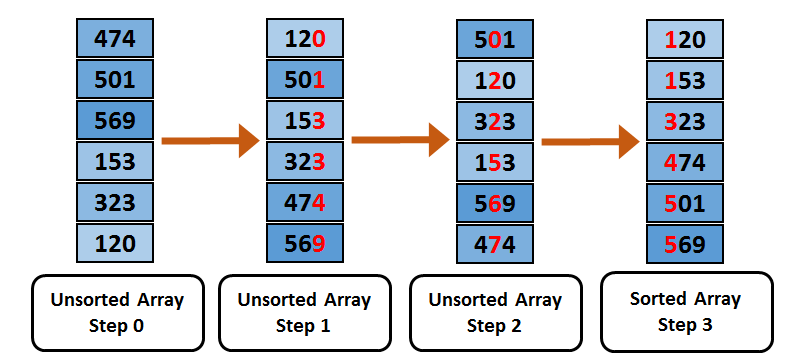
\includegraphics[scale=0.50]{images/figure 14.png}
\caption{Radix Sort of Integer key values.}
\label{fig:ray-sorting}
\end{figure}

%
\subsubsection{Ray Decompression}
%

The first step of the decompression is to apply an exclusive scan operator on the chunk size array. This will give us the indices of the chunks starting positions on the sorted key-index pair array for each pair. With this information we create 2 arrays, the skeleton array and the head flags array. The skeleton is initialized with 1s and the head flags array is initialized with 0s, like we did earlier for the compression. The skeleton array is populated using the output of the exclusive scan that we applied to the chunk arrays, meaning that for each value in the scanned array we alter the corresponding position of the skeleton array with the corresponding chunk base.The head flags array is also marked at the same time with 1s in the same positions that we altered in the skeleton array.After populating both the skeleton and head flags arrays we apply an inclusive segmented scan to them which will give us the sorted key-index pairs that we need for the next step, the hierarchy creation (see figure~\ref{fig:ray-decompression} below).

\begin{figure}
\centering
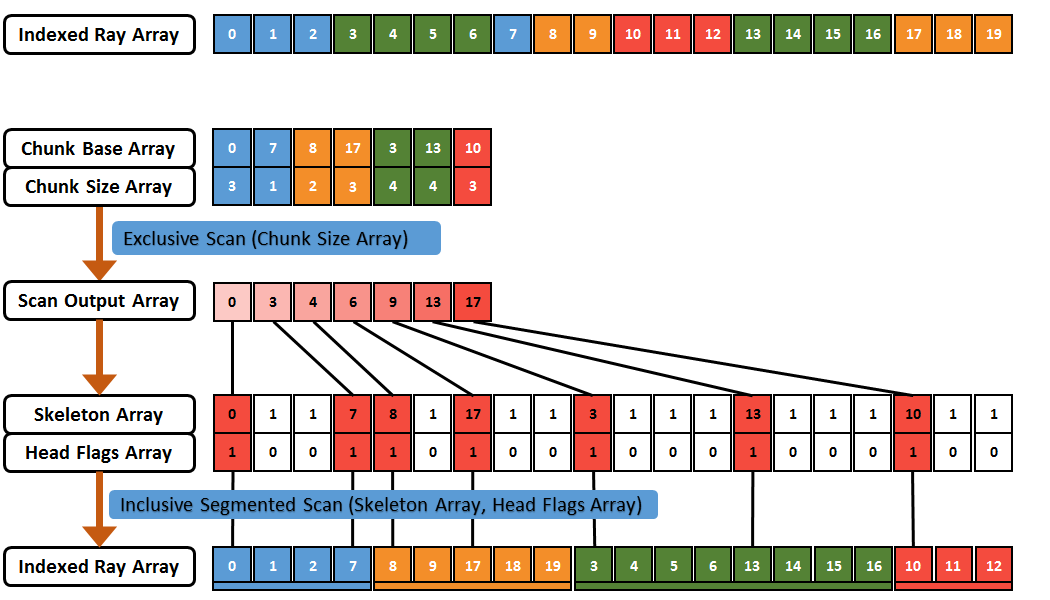
\includegraphics[scale=0.45]{images/figure 11.png}
\caption{Ray Chunk Decompression from Chunks using parallel primitives.}
\label{fig:ray-decompression}
\end{figure}

%
\subsection{Hierarchy Creation}
%

\begin{figure}
\centering
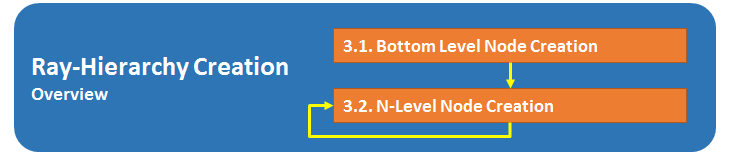
\includegraphics[scale=0.60]{images/figure 4.png}
\caption{Ray-Hierarchy Creation Overview.}
\end{figure}

With the sorted rays we can now proceed to the creation of the actual hierarchy. Since the rays are now sorted according to their coherency the hierarchy will be much tighter in the lower levels of the hierarchy, giving us smaller intersection candidates.
Each node in the hierarchy is represented by a sphere and a cone. (see figures~\ref{fig:bounding-spheres} and~\ref{fig:bounding-cones} below).  The sphere contains all the origins on the rays in the node and the cone also contain the ray itself. This structure  is stored with 8 floats, the spheres center and radius and the cones direction and spread angle.The construction of the hierarchy is done in a bottom-up order, meaning that we start with the leaves, which have a sphere with radius equal 0 and a cone with spread angle equal to 0 as well. The upper levels of the hierarchy are created by calculating the union of the child nodes (in this particular case, each node has 4 children). It is important to note that each ray needs to store the pixel that it corresponds to since after the sorting step the rays are not in their original order so we need a way to map them back to the screens pixels. It is also worth noting that since the hierarchy is in no way tied to the triangles positioning in the scene it does not matter at all for the hierarchy itself  if the scene is dynamic or static.

\begin{figure}
\centering
\begin{minipage}{.5\textwidth}
  \centering
  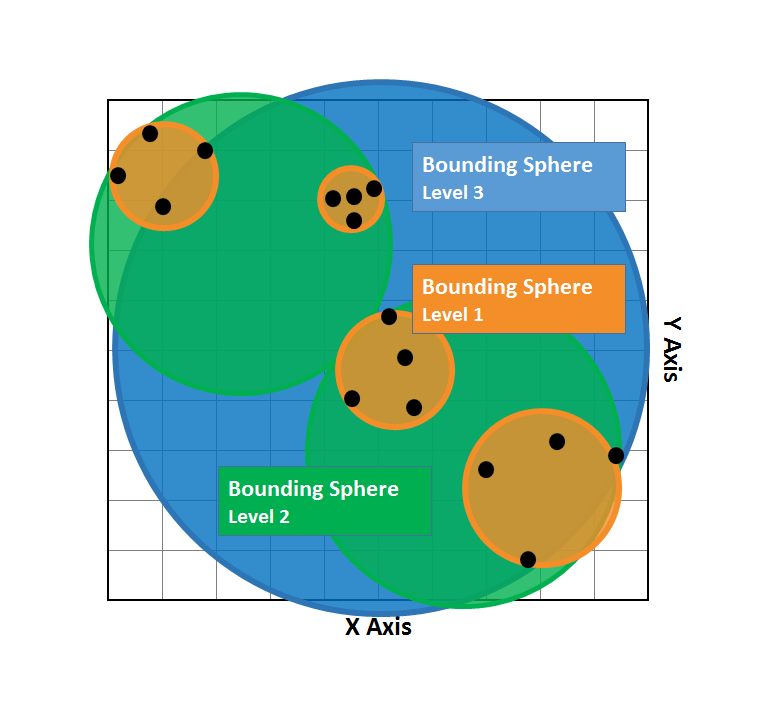
\includegraphics[width=.85\linewidth]{images/figure 12.png}
  \captionof{figure}{Bounding Spheres - 2D}
  \label{fig:bounding-spheres}
\end{minipage}%
\begin{minipage}{.5\textwidth}
  \centering
  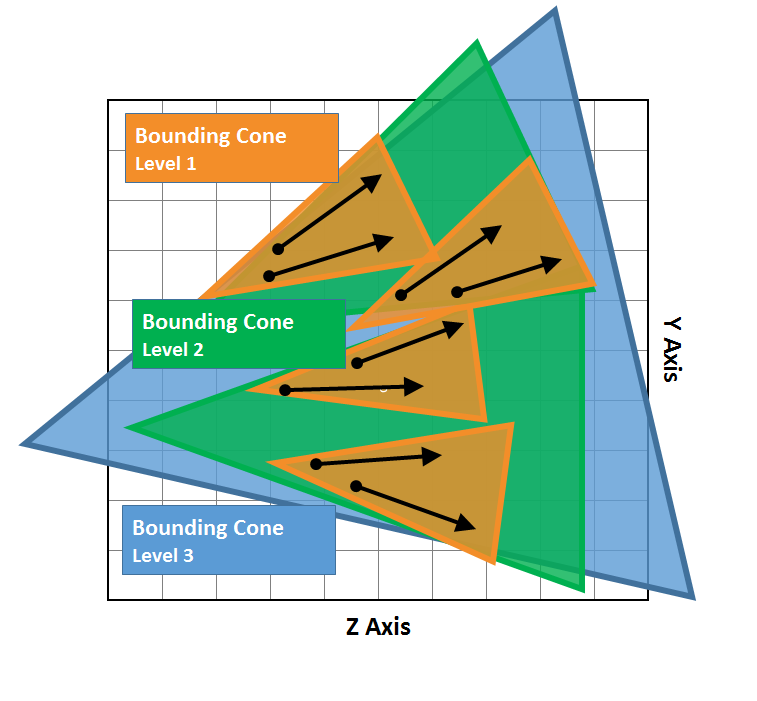
\includegraphics[width=.85\linewidth]{images/figure 13.png}
  \captionof{figure}{Bounding Cones - 2D}
  \label{fig:bounding-cones}
\end{minipage}
\end{figure}

It is also important to note that if the rays are not coherent at all the cones might start to fail. To solve this problem there is a solution that consists of using only the lower levels of the ray hierarchy. Since the rays are sorted before this step, there is a much higher coherency between rays in the lower levels. If we focus on these rays and ignore the higher levels of the hierarchy we will have better results. There is a possibility that we might end up having more local intersection tests but since the nodes in the higher levels of the hierarchy are too big anyway, we would most likely end up having intersections with every single triangle and thus having no real gain from calculating the intersections on these higher level nodes.

%
\subsection{Hierarchy Traversal}
%

\begin{figure}
\centering
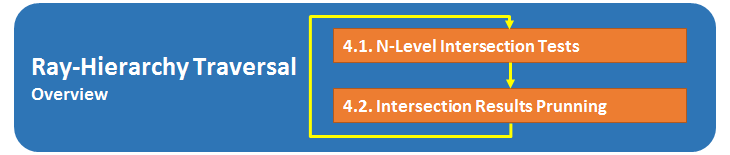
\includegraphics[scale=0.60]{images/figure 5.png}
\caption{Ray-Hierarchy Traversal Overview.}
\end{figure}

Having created the hierarchy all that is left is to traverse it. This is down in a top-down order, intersecting each node with the scenes geometry. Since the top level nodes of the hierarchy fully contain the bottom level nodes, triangles rejected in the top levels will not be tested again for the bottom level nodes. Giving a specific example, we start traversing the hierarchy with the root node. If a certain triangle does not intersect the root node then this means that that specific triangle will not intersect any of its children. Since it is the root node, it also means that no ray in the scene will intersect it so we don't have to test it for intersections any more. After traversing each level of the hierarchy we store the intersection information in a texture so that the children nodes will know which triangles they have to test intersections against. It is also worth noting that the intersection tests being run at this stage are only coarse tests using the triangles bounding sphere since we will have to do the actual intersection tests in the final stage anyway. Since the intersection tests are being run in a parallel manner there is will be a problem regarding empty spaces in the textures that contain the intersection information. These textures need to be pruned by using a stream-reduction pass \cite{RAHStream07} that will remove the empty elements and group the remaining elements together as input for the next level.

%
\subsection{Local Intersection Tests}
%

\begin{figure}
\centering
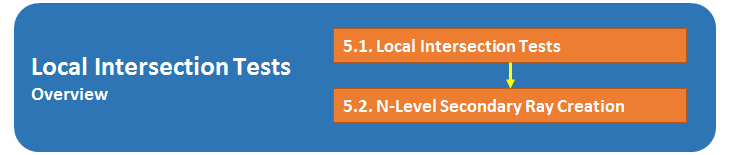
\includegraphics[scale=0.60]{images/figure 6.png}
\caption{Local Intersection Tests Overview.}
\end{figure}

After traversing the hierarchy we will have a list of triangle ID and ray ID pairs, the candidates for the local intersection tests. In this final step all that's left is to find out which one is the closest intersection triangle for each ray and accumulate shading. Depending on the depth that we want for the algorithm we might need to output another set of secondary rays. Since the algorithm is generic, all that's necessary is to output these rays and return to the Ray-Sorting step.

%
\subsection{Shadow Rays}
%

While not necessarily a step in the algorithm, it is important that it is capable of rendering soft shadows. In the rasterization step the output consists of the secondary rays origin, reflection direction and refraction direction. I did not mention shadow rays in this step but since we have the rays origin all we have to do is to trace rays to the light sources and calculate the necessary intersections. The shadow rays are actually very coherent since they all have the same origin and very similar directions if we consider each light source as a grid to which we will trace the several shadow rays, which in turn means that the hierarchy can handle shadow rays very well.

\begin{figure}
\centering
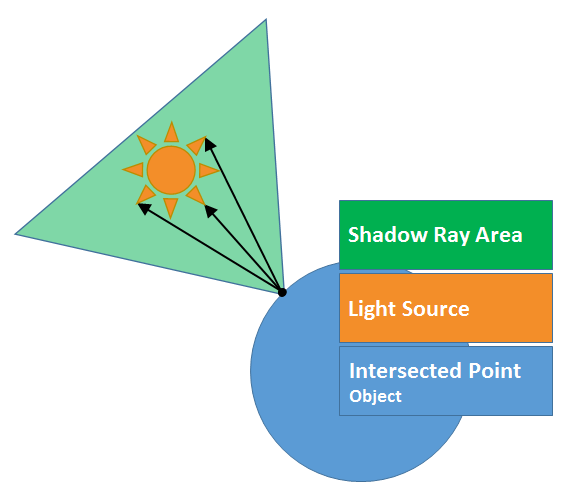
\includegraphics[scale=0.40]{images/figure 16.png}
\caption{(Soft) Shadow Rays}
\end{figure}

%
\subsection{Ambient Occlusion}
%

Like the shadow rays, ambient occlusion are not a step but they are also important to render photo-realistic scenes. Ambient occlusion consists of tracing several rays in an hemisphere above an intersection point. These rays are coherent locally but globally they are hard to bound with cones. This is essentially the same problem that i noted in the hierarchy creation section in which rays might not be coherent enough globally for the upper levels of the hierarchy to be effective. The solution for this problem is the same as the one as I indicated previously, which is to ignore the higher level nodes of the hierarchy and simply start traversing it from a lower level.

\vspace*{-20pt}

\begin{figure}
\centering
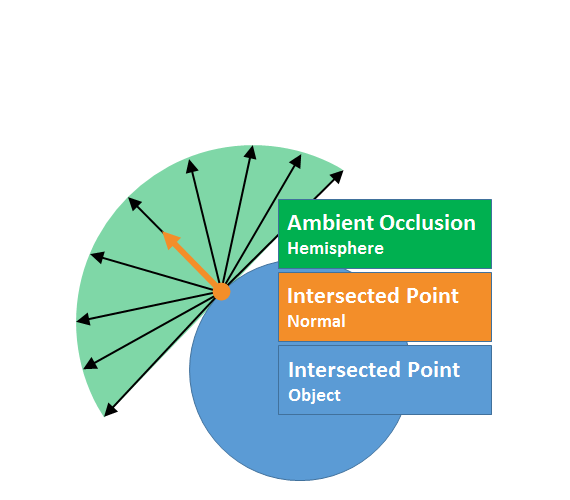
\includegraphics[scale=0.40]{images/figure 15.png}
\caption{Ambient Occlusion}
\end{figure}

\vspace*{-20pt}

%
\subsection{Preliminary Analysis}
%

Although it is hard to analyze the algorithm without actually benchmarking and testing it against different scenes, the modifications I introduced work well with the underlying algorithm. The objective of the Ray Sorting in its original paper by Garanzha and Loop \cite{GaranzhaLoop10} is to create tighter bundles of rays in order to reduce the local intersection tests. Adapting the sorting to the ray-space hierarchy by Roger et al. \cite{Roger07} will help in creating a tighter hierarchy while still keeping the benefits of the cone-sphere structure intact. One of the original problems of Roger et al. \cite{Roger07} algorithm is that at the top levels of the hierarchy the structure itself might fail given rays that are extremely incoherent. However if we start traversing the hierarchy from a lower level this problem will be mitigated (the ray sorting actually makes this even more true since the rays will be ordered by their coherency). We get the  reduced number of intersection tests that we normally would from the higher levels but since the hierarchy would be too loose it is likely that we would end up having almost no benefits at all from traversing the top levels anyway. My solution like Roger at al. \cite{Roger07} leaves room for improvement specifically by combining the ray-space hierarchy with an object-space hierarchy.

%
\section{Evaluation Metrics}
%

%
\subsection{Rays per Second}
%

Since this is a Ray-Tracing project it is necessary to evaluate how many rays per second the algorithm can process. This is the most important metric for the algorithm since it will determine its performance. All the other usual metrics like frames-per-second depend on the number of rays we can process. If we increase the resolution of the screen this will also mean that we need to be able to output the extra number of rays necessary to keep up the performance.

%
\subsection{Intersection test reduction}
%

The main improvement I tried to apply to the original algorithms i based myself on was the reduce the number of intersection tests. That means this metric is very important to measure the success or failure of my solution. I will compare the number of intersections without the Ray-Sorting addition and without the Rasterization steps to the number of intersections with the full algorithm and measure percentage-wise how much my solution reduced these tests.

%
\subsection{Improvements compared to the original algorithm}

It will also be important to compare the algorithm with and without the Ray Sorting step since this is the biggest change that I'm proposing to implement. If the algorithm with the Ray Sorting step is faster than the original one then I can state that there was in fact an improvement and that the sorting does help reduce the number of intersection tests and in turn make the algorithm more efficient. If there isn't an improvement then it might mean that the overhead of the whole sorting process is too significant or that the sorting does not affect the number of intersection calculations in a meaningful way.
%

%
\section{Planning}
%

The planning of the tasks and estimated time that it will take to complete them are represented on the table below. It is important to note that since these are estimated times it is possible that some tasks will take less time and others will take more time, especially the ones concerning the interoperability between OpenGL and CUDA since it is not extremely well documented yet.
The time window is assumed to start on the 1st of February end on the 1st of June. It is also worth noting that each of the tasks involves adding functionality to the previous task.

\begin{table}
\centering
\begin{tabular}{c c c}
\hline\noalign{\smallskip}
Task & Estimated Duration & Estimated Dates \\ \hline\noalign{\smallskip}
Naive Ray-Tracing & 1 week & 1\textsuperscript{st} February to 7\textsuperscript{th} February\\
Rasterization & 2 weeks & 8\textsuperscript{th} February to 21\textsuperscript{st} February\\
Ray Hierarchy & 4 weeks & 22\textsuperscript{nd} February to 21\textsuperscript{st} March\\
Ray Sorting & 4 weeks & 22\textsuperscript{nd} March to 18\textsuperscript{th} April\\
Benchmarking and Testing & 2 weeks & 19\textsuperscript{th} April to 2\textsuperscript{nd} May\\
Msc Thesis & 8 weeks & 3\textsuperscript{rd} May to 2\textsuperscript{nd} June\\ \hline\noalign{\smallskip}
\end{tabular}
\end{table}

In the first task I will implement a naive ray-tracer on the GPU using CUDA and OpenGL. This ray-tracer shouldn't be efficient at all since it will be basically a port of the traditional algorithm without any parallel primitives. It will serve however as a learning platform for me to learn some of CUDAs intricacies and to get accustomed to the platform.
After completing the Rasterization task I should have an application using OpenGLs rasterizer to output the image without any of the ray-tracing secondary effects as well as the initial set of secondary rays. These secondary rays will then be traced using the naive ray-tracer implemented earlier.
For the third step, the Ray Hierarchy I will modify the original naive ray-tracer and adapt it so that it utilizes the hierarchy as well as leaving it structured in such a way that the ray-sorting step can be easily implemented without having to change much of the applications structure. Finally the Ray Sorting step should consist of a simple modification of what is already  implemented. This does not mean that the step itself will be trivial to implement but rather that its integration should be fairly simple. The benchmarking and the writing of the thesis itself should be the final step after everything else is finished.

%
\section{Conclusions}
%

After analyzing several algorithms, some of them being the state of the art, it is clear that there a perfect solution has not been found yet. The main problem is still the number of intersection tests and while there are several approaches have achieved very promising results it still is not enough to bring ray-tracing to real time. The developments over the years in GPUs and the research around GPGPU has helped bring ray-tracing a lot closer but there are still many areas in which improvements can be made.
It is not easy to evaluate my algorithm before actually implementing it but it is safe to say that it will not solve this problem. It should however help mitigate the problem and also leaves some space for future improvement, more specifically by combining an object-space hierarchy with the ray-space hierarchy and thus reducing even more the number of intersection tests.

%
% ---- Bibliography ----
%

\bibliographystyle{abbrv}
\bibliography{references}

\end{document}